\documentclass[tikz, crop, border=5pt]{standalone}
\usetikzlibrary{positioning,backgrounds,fit}

\usepackage{fontspec}
\usepackage{xeCJK}

\setmainfont{NotoSans}[
    Extension      = .ttf,
    UprightFont    = *-Regular,
    BoldFont       = *-Bold,
    ItalicFont     = *-Italic,
    BoldItalicFont = *-BoldItalic
]

\usepackage{color}
\definecolor{indianred1}{RGB}{255, 106, 106}
\definecolor{deepskyblue}{RGB}{0, 191, 255}
\definecolor{palegreen}{RGB}{152, 251, 152}
\definecolor{burlywood}{RGB}{222, 184, 135}
\definecolor{grey}{RGB}{129,130,132}

\begin{document}

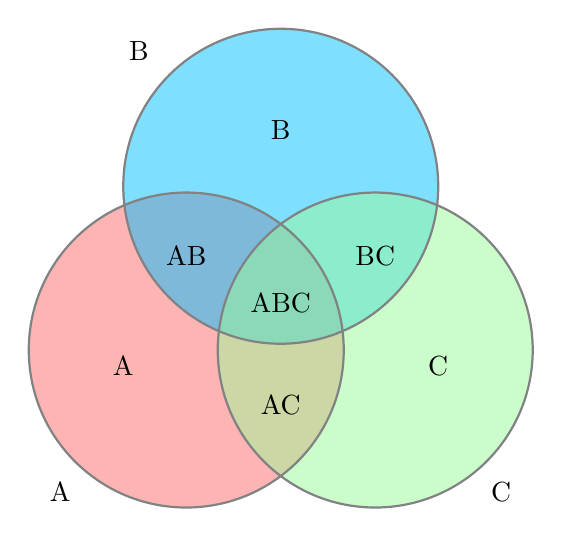
\begin{tikzpicture}
% Basic parameters for circles
\def\radius{2cm}
\def\xshift{1.2cm}
\def\yshift{2.08cm}

% Draw three circles
\begin{scope}[opacity=0.5]
    \fill[indianred1] (-\xshift,0) circle (\radius);
    \fill[deepskyblue] (0,\yshift) circle (\radius);
    \fill[palegreen] (\xshift,0) circle (\radius);
\end{scope}

% Add circle edges
\draw[grey, thick] (-\xshift,0) circle (\radius);
\draw[grey, thick] (0,\yshift) circle (\radius);
\draw[grey, thick] (\xshift,0) circle (\radius);

% Add labels
\node[text centered] at (-2.8, -1.8) {A};
\node[text centered] at (-1.8,  3.8) {B};
\node[text centered] at (2.8,  -1.8) {C};

% Add numbers for exclusive regions
\node[text centered] at (-2,   -0.2) {A};
\node[text centered] at (0,     2.8) {B};
\node[text centered] at (2,    -0.2) {C};

% Add numbers for binary intersections
\node[text centered] at (-1.2,  1.2) {AB};
\node[text centered] at (0,    -0.7) {AC};
\node[text centered] at (1.2,   1.2) {BC};

% Add number for triple intersection
\node[text centered] at (0,     0.6) {ABC};
\end{tikzpicture}

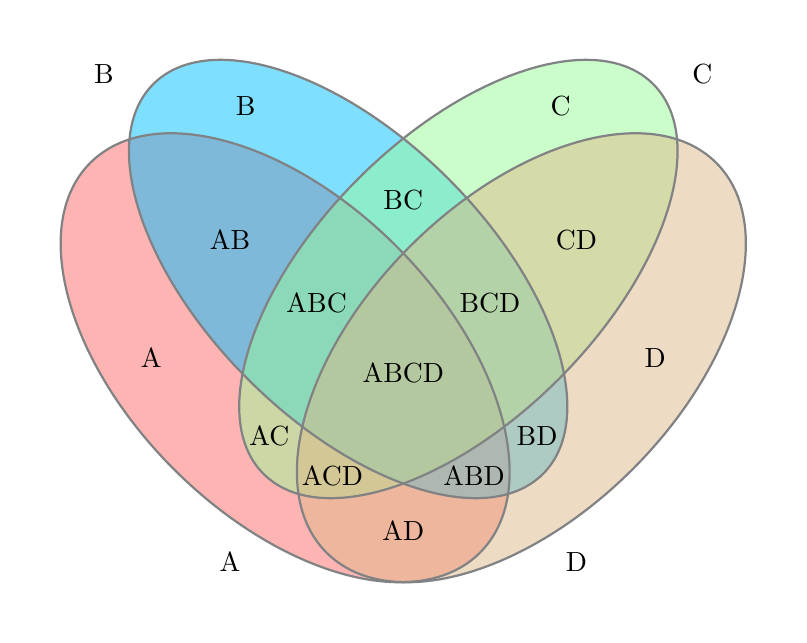
\begin{tikzpicture}
% Basic parameters for ellipses
\def\xradius{3.5cm}
\def\yradius{2cm}
\def\yradiusB{1.8cm}
\def\xshift{1.5cm}
\def\xshiftB{0.7cm}
\def\yshift{1cm}

% Draw four ellipses
\begin{scope}[opacity=0.5]
\fill[indianred1] (-\xshift,0) ellipse [x radius=\xradius, y radius=\yradius, rotate=-45];    % A
\fill[deepskyblue] (-\xshiftB,\yshift) ellipse [x radius=\xradius, y radius=\yradiusB, rotate=-45];    % B
\fill[palegreen] (\xshiftB,\yshift) ellipse [x radius=\xradius, y radius=\yradiusB, rotate=45];      % C
\fill[burlywood] (\xshift,0) ellipse [x radius=\xradius, y radius=\yradius, rotate=45];    % D
\end{scope}

% Add ellipse edges
\draw[grey, thick] (-\xshift,0) ellipse [x radius=\xradius, y radius=\yradius, rotate=-45];
\draw[grey, thick] (-\xshiftB,\yshift) ellipse [x radius=\xradius, y radius=\yradiusB, rotate=-45];
\draw[grey, thick] (\xshiftB,\yshift) ellipse [x radius=\xradius, y radius=\yradiusB, rotate=45];
\draw[grey, thick] (\xshift,0) ellipse [x radius=\xradius, y radius=\yradius, rotate=45];

% Add labels
\node[text centered] at (-2.2, -2.6) {A};
\node[text centered] at (-3.8,  3.6) {B};
\node[text centered] at (3.8,   3.6) {C};
\node[text centered] at (2.2,  -2.6) {D};

% Add numbers for exclusive regions
\node[text centered] at (-3.2,    0) {A};
\node[text centered] at (-2,    3.2) {B};
\node[text centered] at (2,     3.2) {C};
\node[text centered] at (3.2,     0) {D};

%% Add numbers for binary intersections
\node[text centered] at (-2.2,  1.5) {AB};
\node[text centered] at (-1.7, -1.0) {AC};
\node[text centered] at (0,    -2.2) {AD};
\node[text centered] at (0,     2.0) {BC};
\node[text centered] at (1.7,  -1.0) {BD};
\node[text centered] at (2.2,   1.5) {CD};

% Add numbers for triple intersections
\node[text centered] at (-1.1,  0.7) {ABC};
\node[text centered] at (0.9,  -1.5) {ABD};
\node[text centered] at (-0.9, -1.5) {ACD};
\node[text centered] at (1.1,   0.7) {BCD};

% Add number for quadruple intersection
\node[text centered] at (0,    -0.2) {ABCD};
\end{tikzpicture}

\end{document}
